%-------------------------------------------------------------------------------
\section{Eval}
\label{s:eval}
%-------------------------------------------------------------------------------


\begin{figure}[t]
    \centering
    \begin{subfigure}[t]{0.49\columnwidth}
        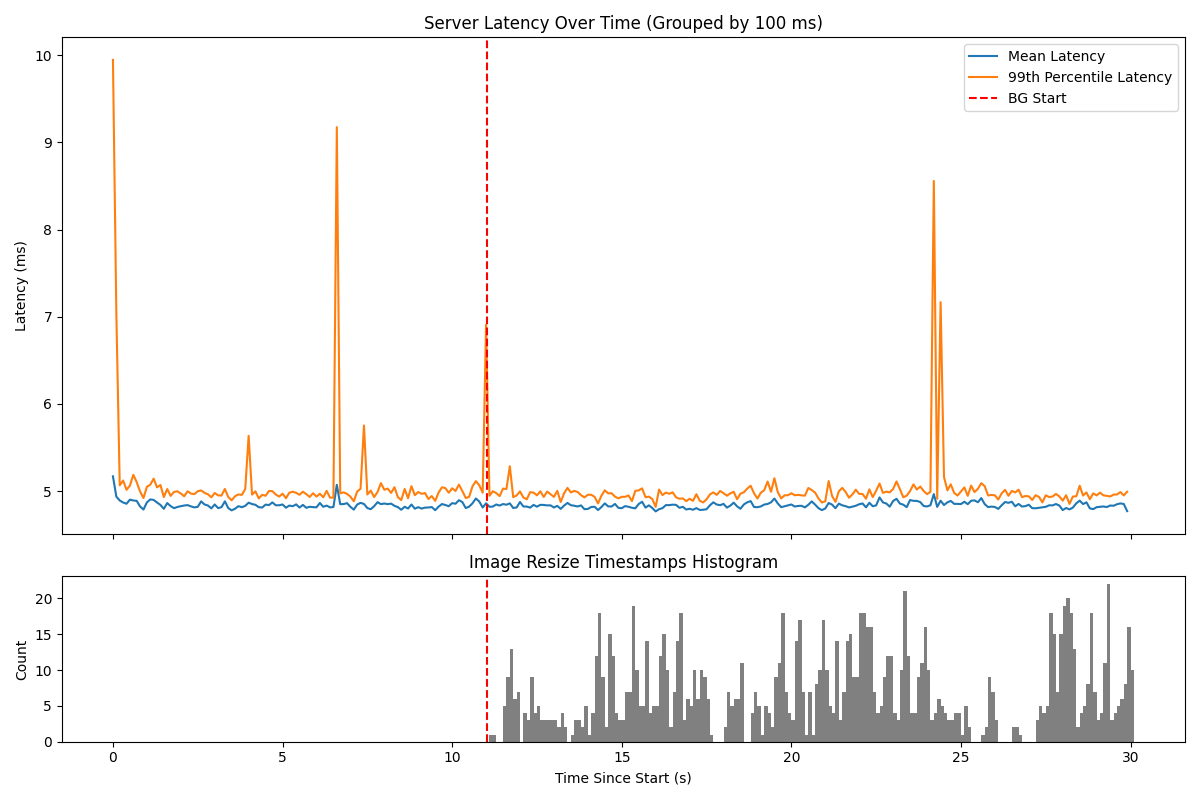
\includegraphics[width=\columnwidth]{graphs/patched-idle-low-two.png}
        \caption{Low load}\label{fig:patched-idle-low-two}
    \end{subfigure}
    \hspace{\fill}
    \begin{subfigure}[t]{0.49\columnwidth}
        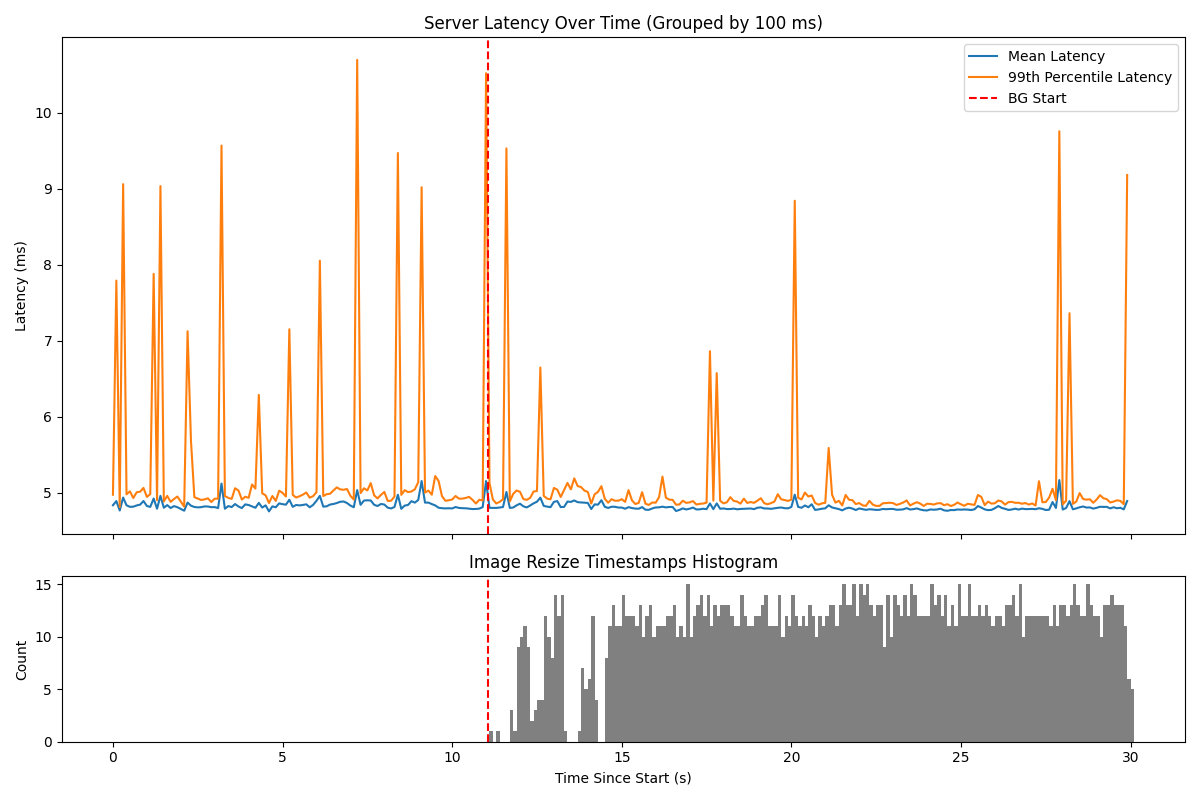
\includegraphics[width=\columnwidth]{graphs/patched-idle-high-two.png}
        \caption{High load}\label{fig:patched-idle-high-two}
    \end{subfigure}
    \vspace{4pt}
    \caption{using a patched \schedidle{} that steals queued \schednormal{}
    tasks before running \schedidle{} ones}\label{fig:patched-idle}
\end{figure}

We can see the resulting performance in figure~\ref{fig:patched-idle}, and see
that as desired the latency of the server remains stable after the background
tasks start. This does not mean that the background task never runs: the lower
graph still shows iterations of image resizing being done. The difference is
that now the background tasks will reliably get interrupted when the LC server
has a request to process.
